% !TEX TS-program = arara
% arara: xelatex: { synctex: on, options: [-halt-on-error] } 
% arara: biber
% arara: biber: { options: [--noremove-tmp-dir] }
% % arara: texindy: { markup: xelatex }
% %% arara: makeglossaries
% arara: xelatex: { synctex: on, options: [-interaction=batchmode, -halt-on-error] }
% arara: xelatex: { synctex: on, options: [-interaction=batchmode, -halt-on-error]  }
% % arara: clean: { extensions: [ aux, log, out, run.xml, ptc, toc, mw, synctex.gz, ] }
% % arara: clean: { extensions: [ bbl, bcf, blg, ] }
% % arara: clean: { extensions: [ glg, glo, gls, ] }
% % arara: clean: { extensions: [ idx, ilg, ind, xdy, ] }
% % arara: clean: { extensions: [ plCode, plData, plMath, plExercise, plNote, plQuote, ] }
%-----------------------------------------------------------------
\documentclass[12pt]{PalisadesLakesBook}
% \geomHDTV
% \geomLandscape
\geomHalfDTV
\geomPortraitOneColumn
%-----------------------------------------------------------------

%\AsanaFonts % misssing \mathhyphen; less on page than Cormorant/Garamond
%\CormorantFonts % light, missing unicode greek
\EBGaramondFonts % fewest pages
%\ErewhonFonts
%\FiraFonts % tall lines, all sans, much less per page, missing \in?
%\GFSNeohellenicFonts 
%\KpFonts
%\LatinModernFonts
%\LegibleFonts
%\LibertinusFonts
%\NewComputerModernFonts
%\STIXTwoFonts
%\BonumFonts % most pages
%\PagellaFonts
%\ScholaFonts
%\TermesFonts
%\XITSFonts

%-----------------------------------------------------------------
\togglefalse{plMath}
\togglefalse{plCode}
\togglefalse{plData}
\togglefalse{plNote}
\togglefalse{plExercise}
\togglefalse{plQuote}
\togglefalse{printglossary}
\togglefalse{printindex}
%-----------------------------------------------------------------
\title{Geology questions}
\author{John Alan McDonald 
(palisades dot lakes at gmail dot com)}
\date{draft of \today}
%-----------------------------------------------------------------
\begin{document}

\maketitle
\PalisadesLakesTableOfContents{7}
%-----------------------------------------------------------------
\begin{plSection}{Introduction}
\end{plSection}%{Introduction}
%-----------------------------------------------------------------
\begin{plSection}{Earth structure}
  \begin{itemize}
    \item Crust-mantle vs lithosphere-asthenosphere?
    \item Upper mantle within lithosphere?
    \item
    $5$ reservoir mixing model for isotope variation in MORB, OIB, and  CRB
    (\citeAuthorYearTitle[chapter 17, Recycling of crustal materials and mantle
    heterogeneity]{Anderson:2007:NewTheory}):
    What's the dimension of the data?
    Is this trivial, or is there some real dimension reduction?
    Does it actually fit in a $4$d simplex?
  \end{itemize}
\end{plSection}%{Earth structure}
%-----------------------------------------------------------------
\begin{plSection}{Plate tectonics}
  \begin{itemize}
    \item Are plates real?
    \item Are ocean and continent plates the same thing?
    \item Just crust or all of lithosphere?
    \item Where are subducting plates/slabs relative to lithosphere/asthenosphere?
    \item Why do plates move?
    \item Is plate motion rigid?
    \item Plate motion relative to what?
    \item Asphericity effects? Could this be a driver?
  \end{itemize}
\end{plSection}%{Plate tectonics}
%-----------------------------------------------------------------

\begin{plSection}{Minerals}
  \begin{itemize}
    \item Is there some rational organizing principle?
    \item Is there a way of plotting mineral attributes that clarifies groups?
    \item Better naming convention, separating rocks and minerals, displaying compositions?
  \end{itemize}

\end{plSection}%{Minerals}
%-----------------------------------------------------------------
\begin{plSection}{Rocks}
\end{plSection}%{Rocks}
%-----------------------------------------------------------------
%-----------------------------------------------------------------
%\BeginAppendices
%%-----------------------------------------------------------------
\begin{plSection}{Typesetting}

This document was typeset using Mik\TeX{} $2.9$ \cite{Schenk:2017:Miktex} 
and {\TeX}works $0.6.5$ \cite{KewLoffler:2017:Texworks} 
on \textsc{Windows} $10$. 
I used \texttt{arara} \cite{CeredaEtAl:2021:Arara} 
to run \texttt{xelatex}, \texttt{biber}, \texttt{makeglossaries},  and
\texttt{texindy: { markup: xelatex }}.
I believe only Mik\TeX\  and {\TeX}works are Windows specific; 
the actual typesetting tools should be usable on Linux and MacOS as well.

See also \cite{Talbot:2012:LatexNovices,Talbot:2013:LatexPhD}.

\begin{plScreen}
{Configuring {\TeX}works for \texttt{arara}.}
{fig:arara}
\centering
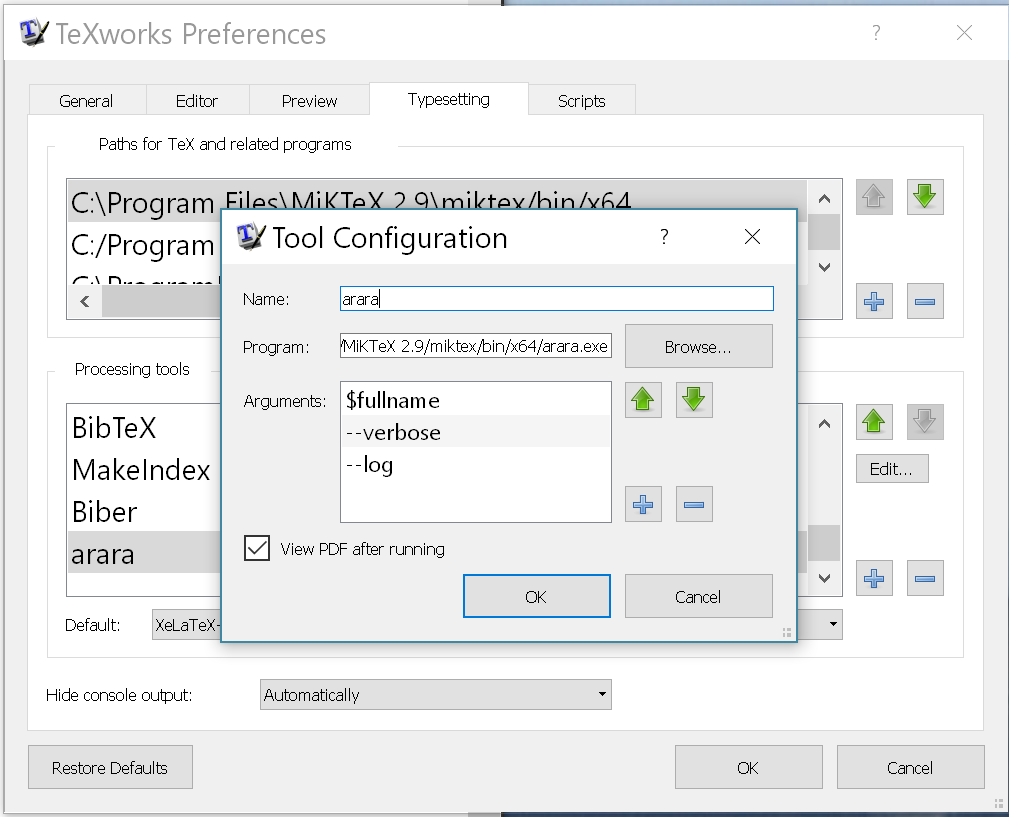
\includegraphics[scale=0.75]{../figs/arara.png}
\end{plScreen}
\vfill
\end{plSection}%{Typesetting}

%-----------------------------------------------------------------
\end{document}
%-----------------------------------------------------------------
